\chapter{Detection of dynamic gestures}

\section{Proposed methods}

The dynamic gesture recognition problem is a problem, where the input data consist of several consecutive positions and orientations of hand and fingers. 
Moreover, the important factor for recognition is the time dependencies between data frames. 
The slower and faster gestures should be recognized as the same dynamic gesture.

The proposed solution utilizes parts of the solution used for recognition of the static gestures.
Each frame of the captured data is described by the same features as in the static recognition part.
The set of features for each frame is then processed by the Hidden Markov Model scheme. 

\subsection{Hidden Markov Model}

Hidden Markov Model is model of a system with Markov property.
The first introduction of HMM comes from the L. E. Baum et. al.\cite{hmmfirst}, who proposed the mathematical background for HMMs.
A HMM can be considered a finite, $N$-element set of states, which are associated with the probability distribution.
The transitions between states are represented by the transition probabilities usually stored in $N\times N$ matrix $T$.
In every state, one of the observation from the finite, $K$-element observation set can be generated with observation probability usually represented by the $N\times K$ emission matrix $E$.
The finite set of all possible observation is called the alphabet.
To fully define the model, the definition of $N$-element vector of initial state probabilities $\Pi$.
Each HMM can be fully defined by the ($T$, $E$, $Pi$).

\begin{figure}[htb]
\centering
 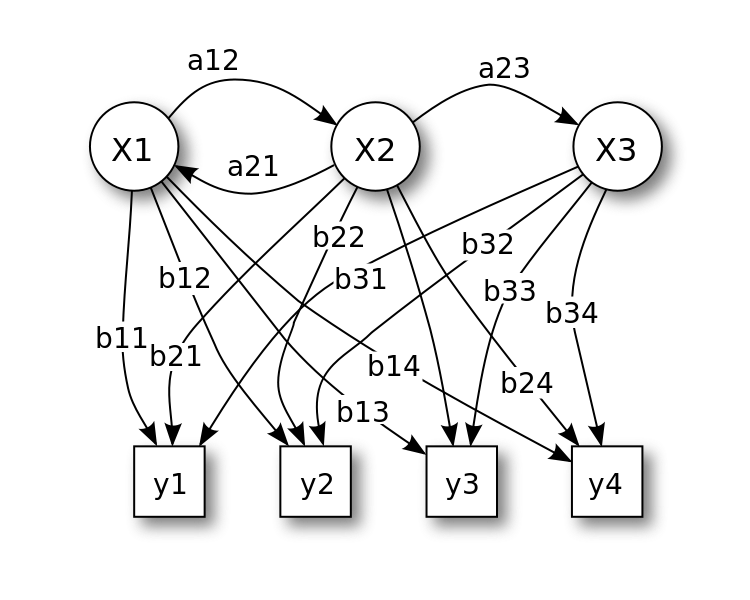
\includegraphics[width=0.8\columnwidth]{figures/HMM_wiki.png}
 \caption[]{Solution blocks of learning and testing parts in task of dynamic gesture recognition\footnotemark}
 \label{dynamicgestureswiki}
\end{figure}

\footnotetext{\url{http://en.wikipedia.org/wiki/File:HiddenMarkovModel.svg}}

The example HMM can be seen at fig.~\ref{dynamicgesturewiki}.
The HMM at the figure consists of 3 states ${X1, X2, X3}$ and 4 possible observations ${y1, y2, y3, y3}$.
The probabilities $a_{ij}$ define the transition probability from state $j$-th to state $i$-th. 
The probabilities $b_{ij}$ define the observation probability of generating $j$ observation while being in state $i$.

The HMM can be understood as a directed graph with two types of weighted vertices. 
This way, each state is represented by one type of vertices while observations can be shown as second type of vertices.
The edges between states contain and are an equivalent to the transition matrix. 
There are no edges between vertices representing observations.
The edges between states and observations are equal to the observation matrix.

$ xx $
There are three main algorithms used with the HMMs:
\begin{itemize}
\item Forward-Backward algorithm, 
\item Viterbi algorithm,
\item Baum-Welch algorithm.
\end{itemize}

The Forward-Backward algorithm is used to find the posterior probability of given states given the set of observations.
For the whole set of state variables $X = {X_i}_{i=1}^{N}$ and a set of observations $o_{1:t} = o_1, o_2,...,o_t$, the algorithm computes the $P(X_i | o_{1:t})$.
The algorithm utilizes a dynamic programming approach, by perfoming 3 steps in a loop: 
\begin{enumerate}
\item computing forward probabilities,
\item computing backward probabilites,
\item computing smoothed values.
\end{enumerate}
Firstly, the forward pass phase for $i=1,..,N$ computes the $P(X_i, o_{1:k})$, where $k$ is smaller than $t$, which represent the probability of ending up in state $X_i$ after first $k$ observations. 
The backward pass computes the $(P(o_{k+1:t}) | X_i)$, which are the probabilities of observing the rest of the observations in state $X_i$.
The smooting part, uses Bayes rule to compute the probability of state $X_i$ given the whole observation sequence:
\begin{equation}
P(X_k | o_{1:t}) = P(X_k | o_{1:k}, o_{k+1:t}) \propto P(o_{k+1:t} | X_k) P(X_k | o_{1:k})
\end{equation}
The time complexity of this algorithm is $O(N^2 T)$, where $T$ is the length of observation sequence and $N$ is the number of possible states.

The Viterbi algorithm is used to find the most likely sequence of hidden states that best explain the set of observations.
The set of those states is usually called the Viterbi path. 
Introduing the sequence:
\begin{equation}
V_{1,k} = P(o_1 | k) * \Pi_k)
\end{equation}
\begin{equation}
V_{t,k} = P(o_t | k) * argmax_{x\in X}(a_{x,k} * V_{t-1,x})
\end{equation}
Finally, the problem can be understood as finding the $argmax_{x\in X}(V_{T,x})$. 
The algorithm time complexity is the same as forward-backward $O(N^2 T)$.

The Baum-Welch algorithm is the algorithm used to find the unknown parameters of the HMM.
For each training example, the algorithms updates the state transition probabilities, observation probabilities in each state and initial probabilities to maximize the likelihood of observation.
Having the set of sets of observations, the algorithm can be used to train HMM to detect the sequences similar to the ones used in learning process.

\begin{figure}[htb]
\centering
 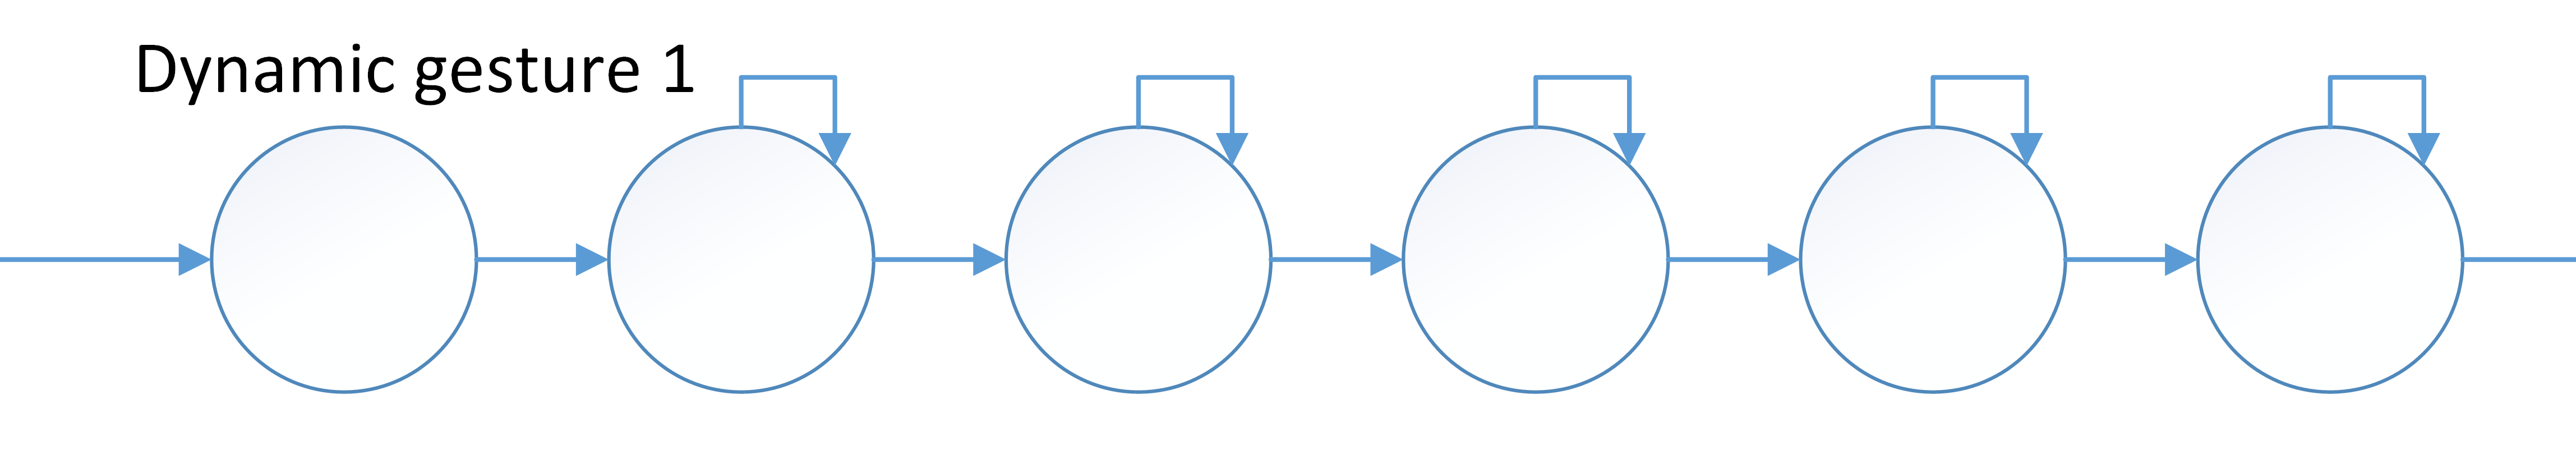
\includegraphics[width=1\columnwidth]{figures/SingleHMM.png}
 \caption{Non-zero state transitions and states of the HMM used to detect single dynamic gesture}
 \label{singlehmm}
\end{figure}

In the dynamic gesture recognition task, we adopted a structure of HMM with state having non-zero transition probabilities to self and to the next state in the sequence.
The proposed structure is presented at fig.~\ref{singlehmm} and was firstly proposed in paper~\cite{hmm}.
The states can be understood as the phases of hand movement and position that happen when the wanted gesture is performed.
The self-transitions are used to model the different speeds of the gestures.
This structure after training process can be used to measure the probability of that the dynamic gesture occured given the set of observations.

\begin{figure}[htb]
\centering
 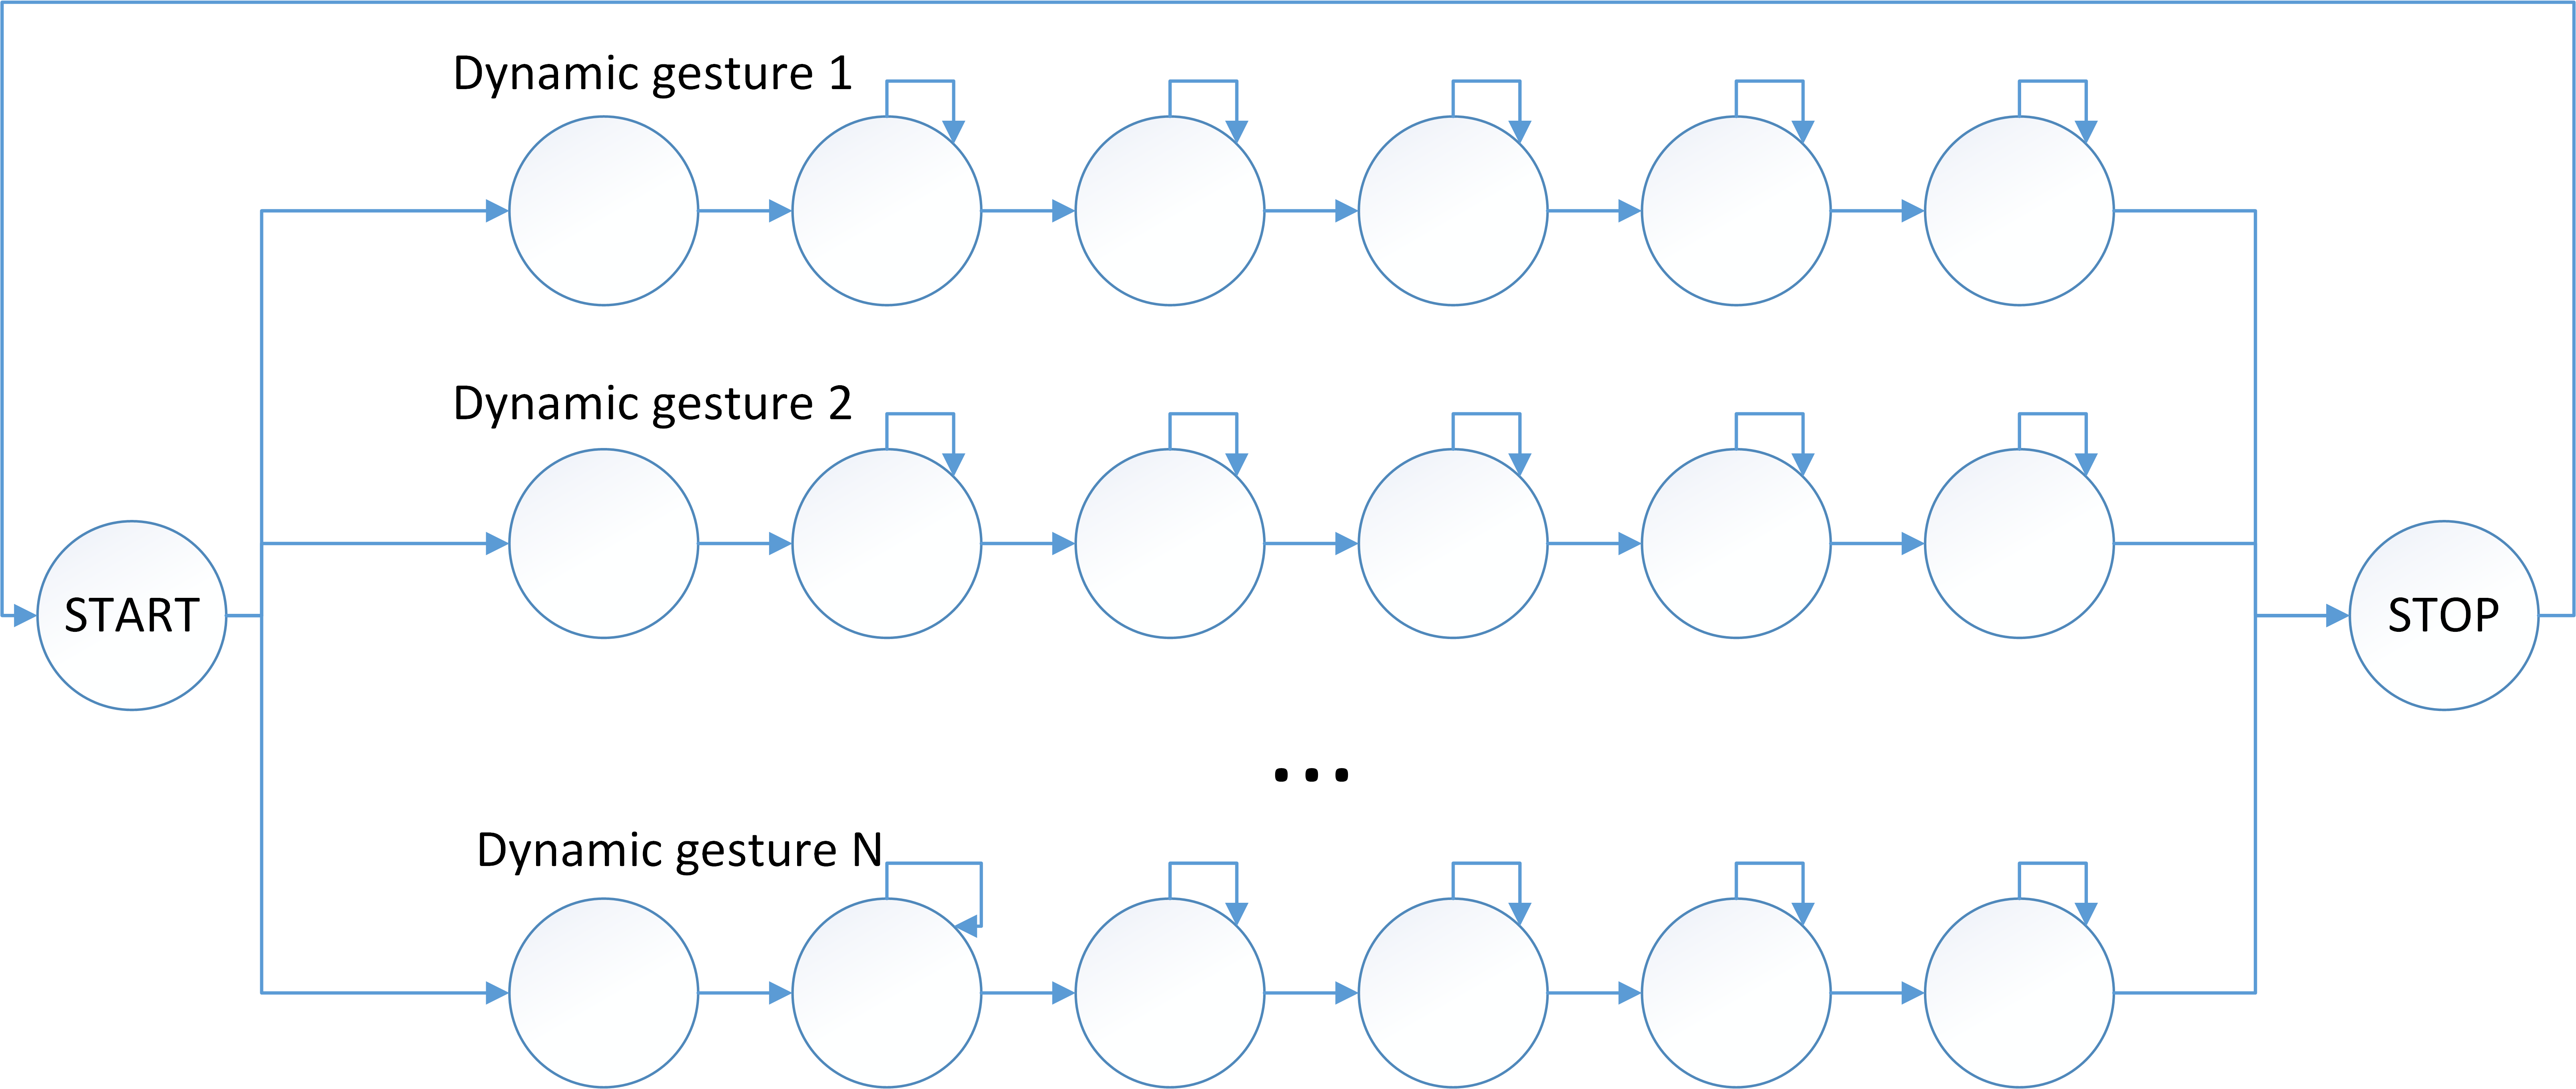
\includegraphics[width=1\columnwidth]{figures/HMM_eng.png}
 \caption{Non-zero state transitions and states for the HMM enabling simulatneous detection of $m$ dynamic gestures}
 \label{HMMstructure}
\end{figure}

Having single dynamic gesture recognition problem modelled as the sequence of $n$ states in which $kths$ state is connected by the edges to the $k$ and $(k+1)$ state and to the all observations.
Having the problem of distinguishing $m$ gestures translates to the $m$ sequential graphs.
The problem of finding if and what dyanmic gesture occured is the problem of finding the probabilities from each $m$ HMM and checking them against preset threshold.
Alternatively, the $m$ HMMs can be combined into one HMM were those single HMMs are treated as parallel paths.
The structure of proposed single HMM is presented at fig.~\ref{HMMstructure}.
Then the recognitnion process is a process of finding, which of the parallel paths is the most probable.
The only remaining problem is the problem of preparing the set of ccured, 1-dimensional observations from the Leap Motion data.

\subsection{HMM observation from Leap Motion data}

Most of the proposed solutions in the literature assume that the observations are 1-dimensional.
There were attempts to expand the HMM to the 2-dimensional observations [], but the raw data from Leap Motion is defined in higher-dimensional that any found solution.
That is the reason, why the need to reduce the dimensionality of the observation of the single hand in the predefined moment in time.

To do this, unsupervised clustering algorithms were introduced. 
For this task we examined 3 methods:
\begin{itemize}
\item Chinese whispers \cite{CW1, CW2},
\item Girvan-Newman clustering \cite{Newman},
\item k-means with additional methods to determine the number of clusters. \cite{kmeans1, kmeans2}.
\end{itemize}

Chinese whispers algorithm is an efficient randomized graph-clustering algorithm, which is time-linear in the number of edges.
The algorithm was proposed in \cite{CW1} and thoroughly examined in Natural Language Processing problems. 
The main advantage of the algorithm is the ability to independently determine the number of classes. 
In tests, we used the implementation available in dLib-ml library\cite{dlib}, which provides multiple machine learning algorithms.

Girvan-Newman clustering is a hierarchical algorithm used to detect clusters in a data represented as a graph.
The algorithm progressively removes edges from the original network until it reaches the maximal number of iterations or the error condition is met.
The solution iteratively calculates the eigenvalues of a created matrix using the power iteration method. 
In case of a complete graph, this algorithm is relatively slow.

The another proposed approach is a k-means clustering algorithm.
The idea for the algorithm comes from polish mathematician Hugo Steinhaus \cite{kmeans1}, but the first practical application has been presented in \cite{kmeans2}.
The algorithms initially randomly selects $k$ starting points and performs iteratively 2 steps utilizing the idea of expected-maximization \cite{expectedmaximization}:
\begin{enumerate}
\item For each data sample the algorithm calculates the distances to $k$ centroids and labels the samples with the label of the centroid with the smallest distance.
\item For each class, the algorithm recalculates centroids position to the averaged position of all samples belonging to class.
\end{enumerate} 
The algorithm stops after maximum number of iterations or when the change between consecutive iterations is smaller then defined epsilon.
Unfortunately, the algorithm requires the knowledge of the number of expected classes.
Although there exists a heuristics methods aiding in correctly choosing the number of classes. 
One of those methods is plotting the error sum of squares (SSE) within classes against the number of chosen classes. 
In this plot the drastic drop of SSE is sough and the number of classes it happens is considered a good choice.
Another, more formal approach introduces the measure of dissimilarity and is called Silhouette width \cite{silhouette}.
Declaring $a(i)$ as the average dissimilarity with all the other data within the same cluster and $b(i)$ as the lowest average dissimilarity to any other cluster which $i$ is not a part of, we can write a measure:
\begin{equation}
s(i) = \frac{b(i) - a(i)}{\max{\{a(i),b(i)}\}}
\end{equation}
The big value of $s(i)$ implies good clustering, while small value of $s(i)$ suggests that the number of classes was not properly chosen.





\begin{figure}[htb]
\centering
 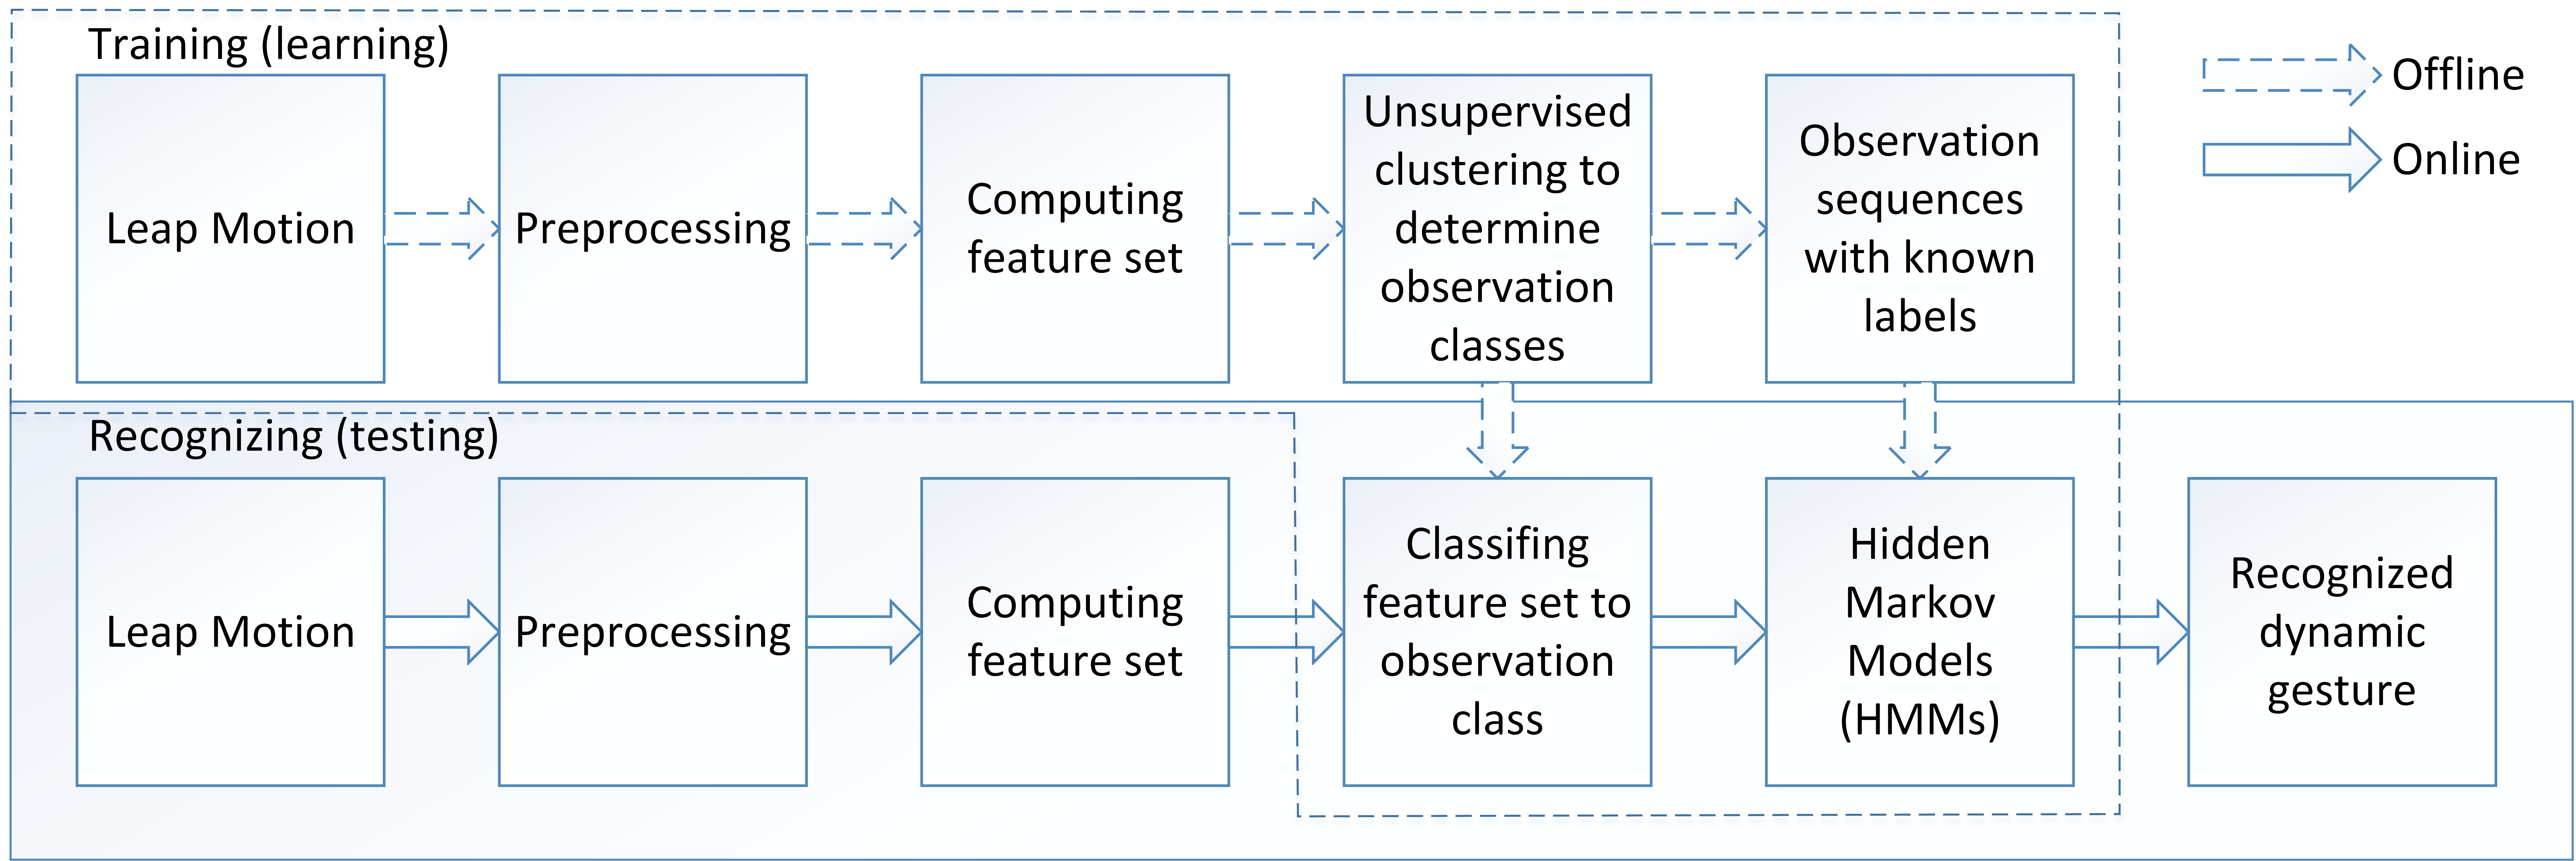
\includegraphics[width=1\columnwidth]{figures/DynamicGestures.png}
 \caption{Solution blocks of learning and testing parts in task of dynamic gesture recognition}
 \label{dynamicgesturesflow}
\end{figure}

Finally, the whole processing flow has been designed and is presented at fig.~\ref{dynamicgesturesflow}.
The whole solution consists of two parts: offline learning and online recognition.
For learning, the raw data is preprocessed and then the feature are extracted. 
Similarly to the static gestures, the features set were computed. 
In training part, those features are extracted from all recorded positions for all dynamic gestures.
Then one of the unsupervised clustering algorithms is used to find the classes of observations.
Knowledge of the classes is used to represent each dynamic gesture as a series of one-dimensional observations.
After that for each dynamic gesture, the corresponding HMM is learned by running the Baum-Welch algorithm on the sequence of observations.
To complete, the training process, the HMMs are combined into one HMM.

In the online working, the raw data from leap motion is preprocessed, then each frame is labelled accordingly to the classes learnt by the unsupervised clustering algorithm.
The next step include providing the set of observations to HMM and running the Viterbi algorithm.
The Viterbi algorithm finds the most likely sequence in one the parallel paths, which informs us about the number of the found gesture. 
If the likelihood is above preset threshold, the gesture is assumed to be correctly recognized.


\section{Evaluation methodology}

To evaluate the quality of recognition achieved by proposed processing pipeline, 8 dynamic gesture were chosen for which the data was recorded.
For each of those gestures, we recorded 120 samples (30 samples per each author).
The recorded data were in different positions, with different speed to measure the wanted invariance.
The chosen dynamic gestures are:
\begin{enumerate}
\item ``number 8'' -- it's a number 8 made by one finger in the air,
\item ``letter Z'' -- it's a letter Z made by one finger in the air,
\item open hand with 5 fingers going down in the direction of the sensor,
\item ``clearing'' -- open hand moving left and right and simulating the movement of clearing the screen,
\item circle made by one finger in the air
\item ``letter A'' -- a letter A made by one finger in the air,
\item ``gun'' -- only the thumb and the index finger are not in the fist. The hand moves up simulating the movement during the firing from the gun.
\item ``swipe from right'' -- moving the hand from right to left, used e.g. in smartphones to move something out of the current view.
\end{enumerate}

To test the proposed approach, similarly to the static gesture recognition problem, the $120\times8=960$ samples were divided into training and testing group. 
The part of the gestures recorded by Katarzyna were used to find the proper number of clusters than could be used by form the observations for the HMMs. 
The training set was used to train each HMM separately on the training data of each gesture. 
To prevent overfitting of the data and achieve the measure when the training process should be stopped, the k-fold cross validation was utilized. 


\section{Experiments}



The performed experiments started with testing the unsupervised clustering methods to determine the correct number of observations.
Based on the successful static gesture recognition, each of the hand poses was represented by the vector of values containing:
\begin{itemize}
\item number of detected fingers,
\item 5 greatest angles between the finger tip vector and palm normal,
\item 5 greatest angles between the fingers tip vectors,
\item 5 greatest distances between the tip positions of fingers.
\end{itemize}
In order to compare different hand poses, the distance function was introduced as the L2 norm between feature vectors:
\begin{equation}
d(x,y) = \sqrt{ \sum_{i=1}^{16} (x_i - y_i)^2 }
\end{equation}
The Chinese whispers and Girven-Newman uses the similarity function, which was defined as: 
\begin{equation}
s(x,y) = \frac{1.0}{ \max{\{d(x,y), eps\}}}
\end{equation}
where $eps$ was the numerical epsilon.

For the Chinese Whispers and Girven-Newman clustering the typical parameters from dlib-ml library were used --- the Chinese Whispers maximal iterations were set to $100$, while the Girven-Newman was run with maximal iterations equal to $2000$ and precision eps set to $1e-4$.
For the SSE analysis for different cluster number, the publicly available script was used\cite{SSE}. 
The script automatically calculates the k-means clustering algorithm for chosen range of $k$ values and presents the figures, which can be a help in determining the correct number of classes.
For the Silhouette width analysis own, R script was written.



\begin{figure}[htp!]
\centering
 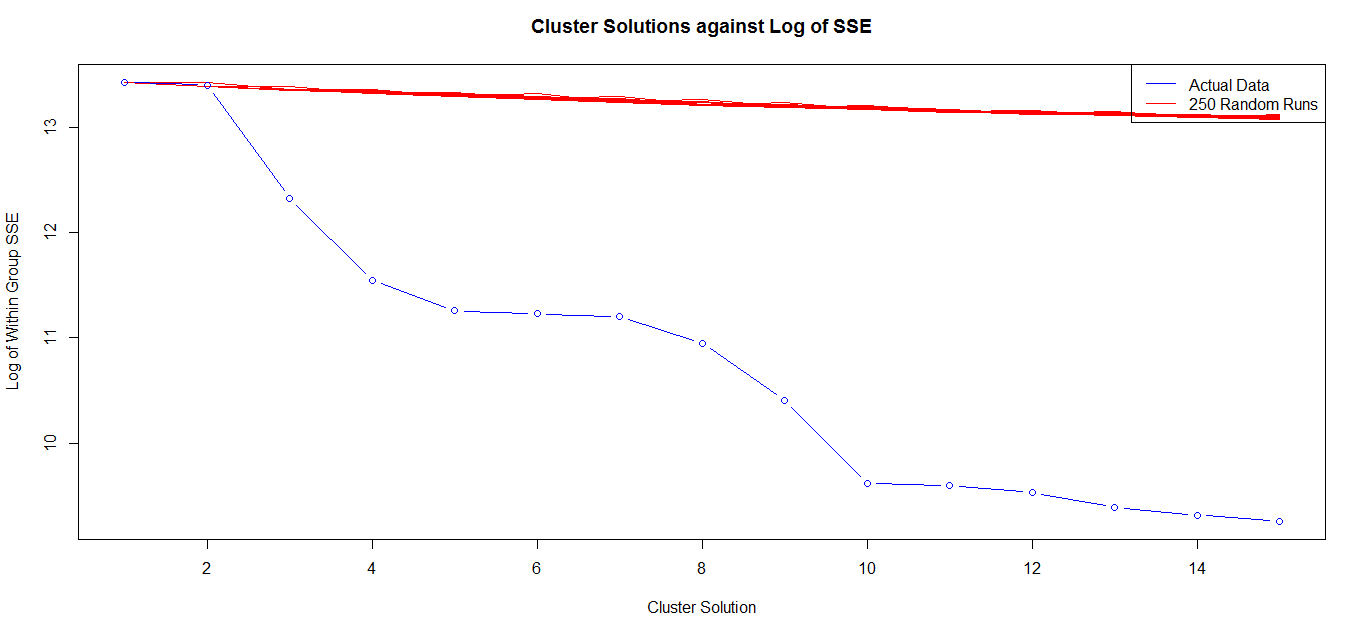
\includegraphics[width=1.0\columnwidth]{figures/SSE1.png}
 %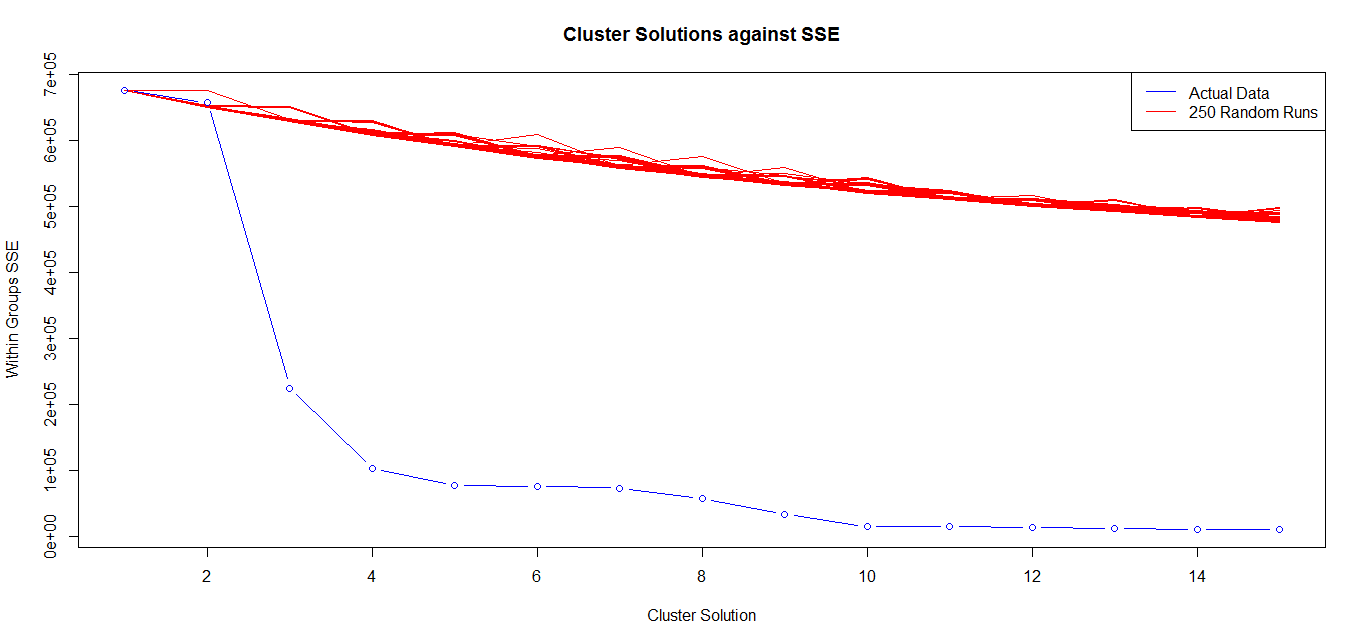
\includegraphics[width=0.7\columnwidth]{figures/SSE2.png}
 %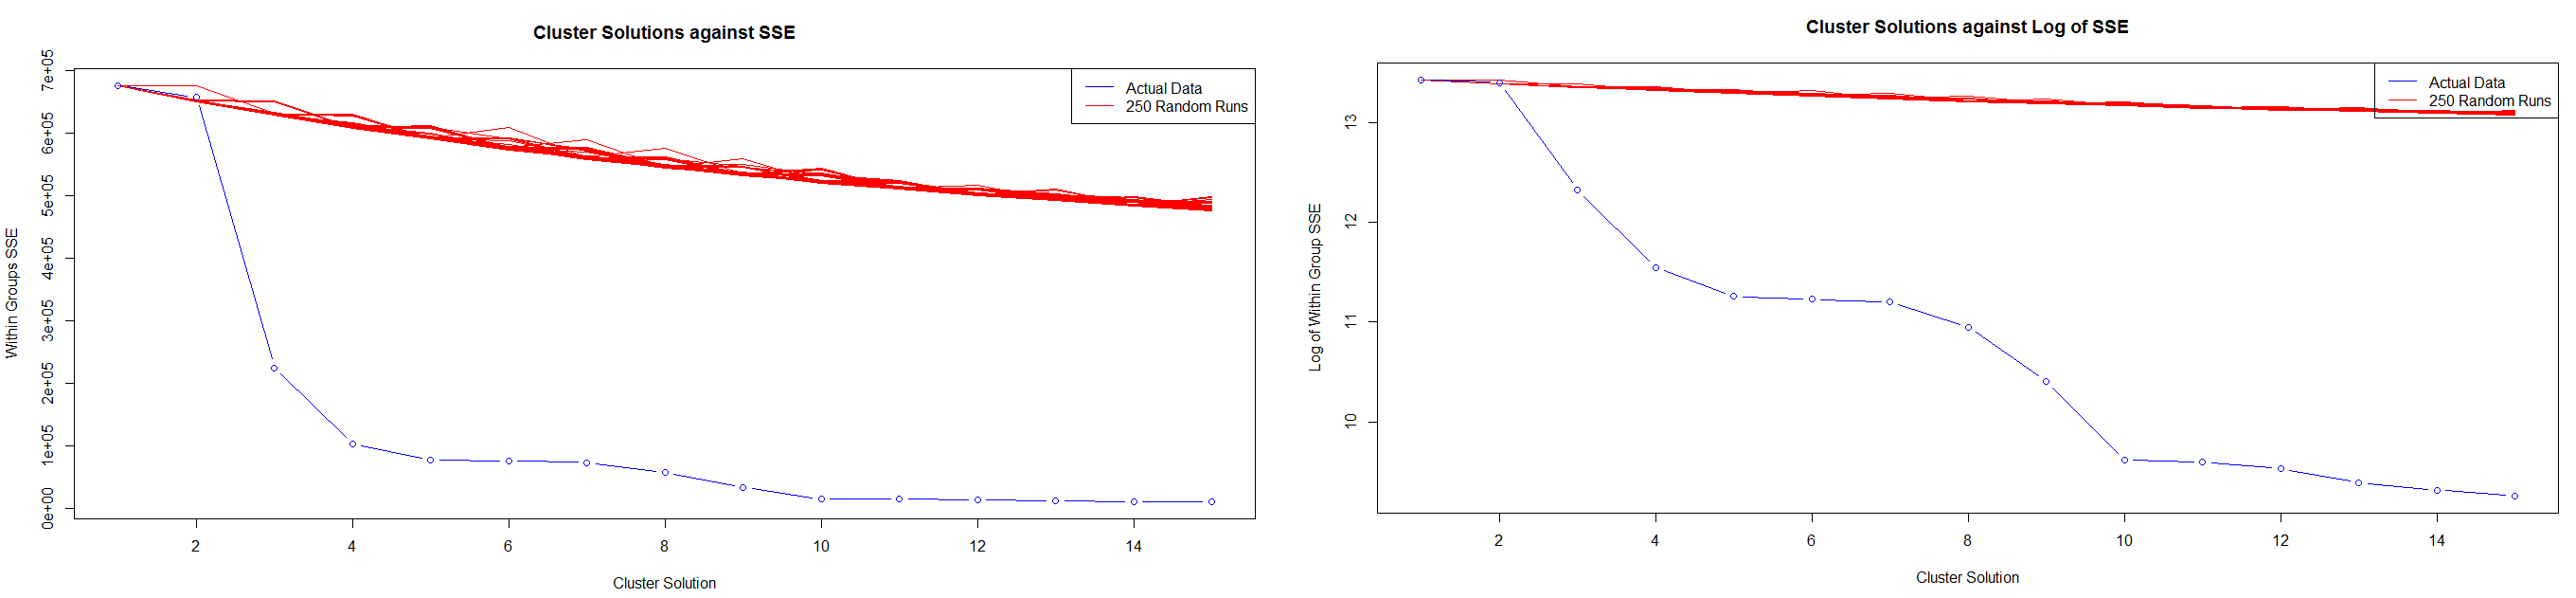
\includegraphics[width=1\columnwidth]{figures/SSE.png}
 \caption{Different representations of SSE as a function of number of clusters for the k-means algorithm}
 \label{dynamicSSE}
\end{figure}

The SSE analysis usually does not yield the direct answer.
The toll provides several plots, but the most interesting one is presented at fig.~\ref{dynamicSSE}. 
Looking at this plot, there is a significant drop in SSE for the cluster number equal to $5$ and $10$.
It is expected that either of those numbers is the correct choice when it comes to the number of classes for k-means algorithm.



\begin{table}[ht]
 \caption{Comparison of suggested number of clusters for the dataset containing all positions of hand in all dynamic gesture recordings made by Katarzyna}
 \label{clusterwyn}
    \begin{tabular}{ccccc}
    \hline
     & Girven-Newman & Chinese whispers   & SSE vs clusters & Silhouette width  \\ \hline
    recordings \\by Katarzyna          & x      & xx & 5 or 10     & xx     \\ \hline
    \end{tabular}
\end{table}

The proposed values of clusters for different methods are presented in the table~\ref{clusterwyn}.



********8
*********88
*DYNAMICZNE TESTY
********88
********


